\newpage
\section{Part 2}
Three various baby and noise sounds were provided by the institute. The sample
frequency for all of the recorded files are 8 kHz. In Figure
\ref{fig:baby_spec} and Figure \ref{fig:noise_spec} the frequency spectrum is
plotted for the baby respective noise sounds. Because the energy levels are
unproportionally low for two out of the three audio recordings, an enhanced
plot is displayed in Figure~\ref{fig:enhanced}.  From the plots it can be seen
that the baby freqency interval is between $\sim$ 300-2500 Hz, including cry
and talk, and the noise frequency interval is between $\sim$0-200 Hz and
$\sim$1300-2100 Hz. One way to work with only the desired frequencies is to
create a filter with a bandpass between 300-1300 Hz. 

%\begin{figure}[h]
%  \centering
%  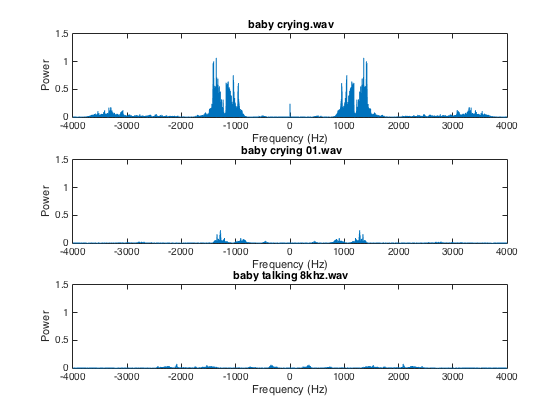
\includegraphics[width=1\textwidth]{sections/freq_spec_baby_linkaxis.png}
%  \caption{Frequency spectrum for baby sound files}
%  \label{fig:baby_spec}
%\end{figure}
%
%\begin{figure}[h]
%  \centering
%  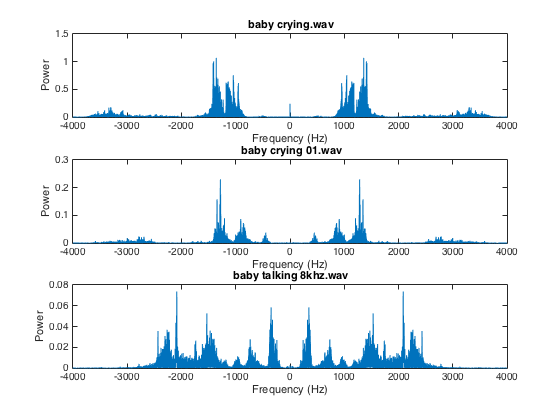
\includegraphics[width=1\textwidth]{sections/freq_spec_babyFix.png}
%  \caption{Frequency spectrum for baby sound files with scaled y-axis}
%  \label{fig:enhanced}
%\end{figure}

\begin{figure}[H]
  \centering
  \begin{minipage}[b]{0.6\textwidth}
    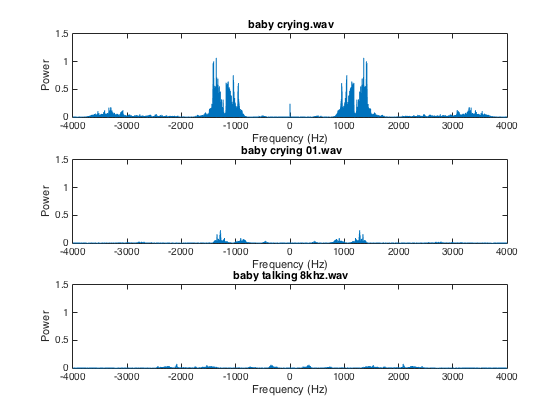
\includegraphics[width=1\textwidth]{sections/freq_spec_baby_linkaxis.png}
    \caption{Frequency spectrum for baby sound}
    \label{fig:baby_spec}
  \end{minipage}
  %\hfill
  \begin{minipage}[b]{0.6\textwidth}
    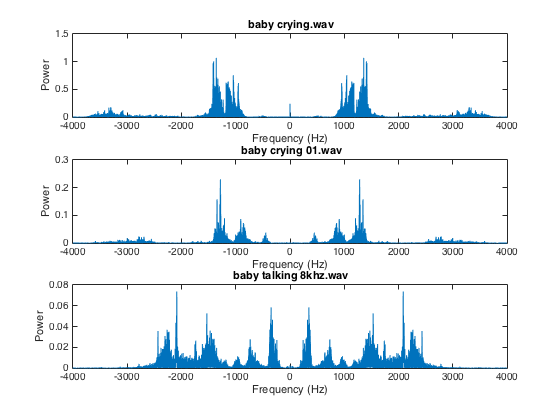
\includegraphics[width=1\textwidth]{sections/freq_spec_babyFix.png}
    \caption{Frequency spectrum for baby sound, scaled y-axis}
    \label{fig:enhanced}
  \end{minipage}
\end{figure}

\begin{figure}[H]
  \centering
  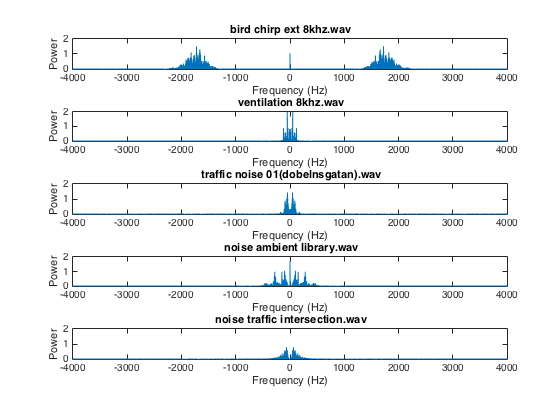
\includegraphics[width=1\textwidth]{sections/freq_spec_noise_2.png}
  \caption{Frequency spectrum for noise files}
  \label{fig:noise_spec}
\end{figure}

\subsection{The algorithms}
A quick and simple algorithm for a BAD application is preferably an algorithm
that measures the energy from the input sound. Another benefit of using this
technique is that the implementation in Android OS may be easier for a novice
application developer.  Mathematically described, the power equation, which is
close relationship to energy, is given by the following formula: 
\[
P(n) = \frac{1}{N} \sum\limits_{k=0}^{N-1} x^2(n-k)
\]
Since the BAD application will be performing these power calculations of the
input sound in real-time, it is undoubtedly impossible to implement the
equation above. A solution to the problem is to use the \emph{recursive
averaging} algorithm. It is small and hardware friendly algorithm that
calculates the power of a given input without using too much memory.
Given the equation below,
\[
P(n) = \alpha P(n-1)+(1-\alpha)x^2(n)
\]
instead of performing the calculation for one sample at the time, a predefined
number of samples in blocks, referred to as frames, are squared and summed.
Each frame represents $x^2(n)$. Every result, $P(n)$, is saved to be used as
$P(n-1)$.  The $\alpha$ is a constant between 0 and 1 and is related to the
following formula:
\[
\alpha = \frac{1}{T_{s}F_{s}}
\]
Despite that the $\alpha$ can be derived from the equation, to get the better
results further tweaking and testing is required.  The $\alpha$ value used in
this research, $0.5$, suggests that the new $P(n)$ is equally weighted between
old and new calculations.  The MATLAB code for the simple algorithm can be
found in Appendix B.

The advanced algorithm is based upon the same, \emph{recursive averaging},
algorithm but before calculating the power of the input sound, the signal
is first filtered through a Butterworth bandpass filter to remove unwanted
frequencies. Butterworth filter, because is gives the least amount of
ripple in the bandpass. By having the noise frequencies suppressed, more
precision is acquired for finding baby activity. The MATLAB code for the
filter can be found in Appendix A.

\begin{figure}{H}
  \centering
  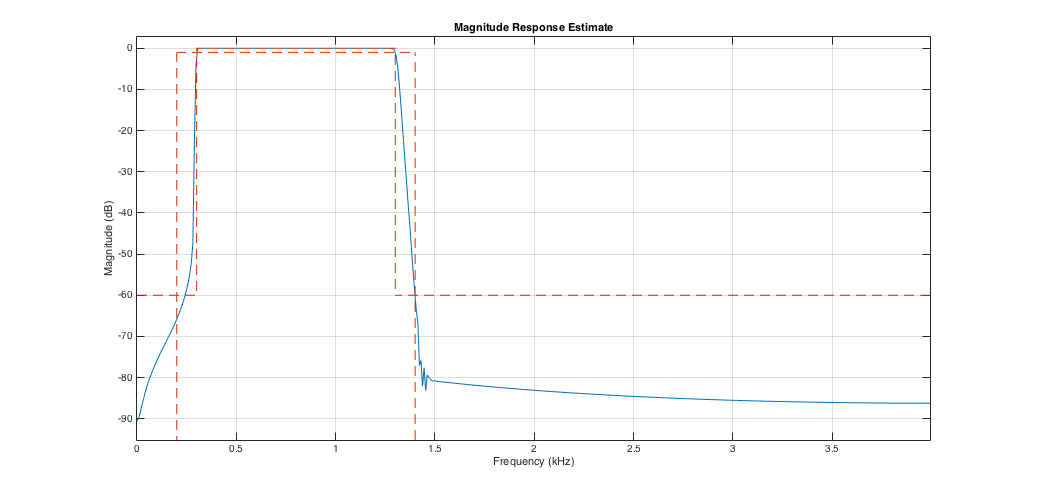
\includegraphics[width=1\textwidth]{sections/butt_pass_est.png}
  \caption{Butterworth 300-1300 Hz bandpass filter}
  \label{fig:butt_pass}
\end{figure}

\subsection{Evaluation and performance}
To evaluate and test the performance of the simple and advance algorithm new
sound files were created, the three provided baby sound files created the
based. The goal was to make the alarm go off with the sound that the baby
caused, in clean and noisy configurations.  For each baby sound file, three new
sound files were created to mislead the algorithms. The MATLAB code for this
can be found in Appendix C.  Giving three sets of 4 different test
configurations, each set contained the following files: 

\begin{enumerate}
  \item clean baby sound without any noise
  \item simulate early mornings, bird and ventilation noise added to the base
  sound
  \item simulate daily environment, all noise files added to the base sound
  \item simulate \emph{extremely} noisy environment, all noise files amplified
  and added to the base sound
\end{enumerate}

As can be seen from Figure \ref{fig:bc1_simp_crop}, the green horizontal line
indicates the threshold value. The red circle indicates where the alarm
has been set off, when the algorithm has notified the user of baby activity. If
the algorithm failed to set off the alarm, the red circle is placed in the
origo. In this test environment the alarm was set off after five frames
successfully breached the threshold value.

\begin{figure}[H]
  \centering
  %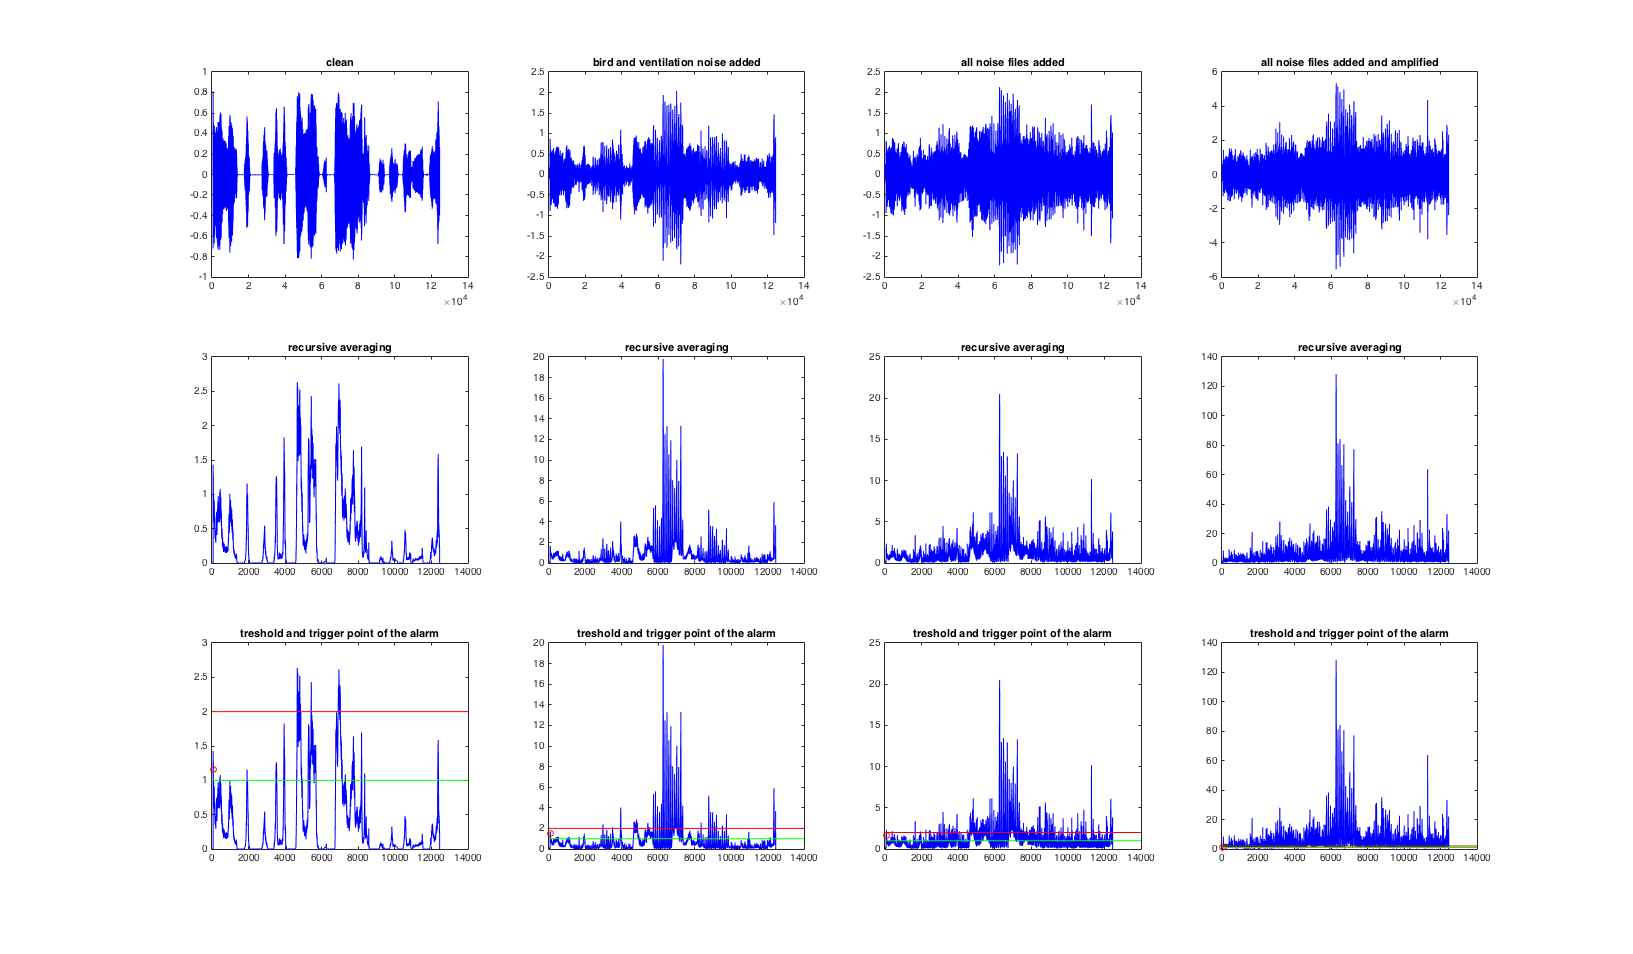
\includegraphics[width=1\textwidth]{sections/newFigures/bc1_unfilt.png}
  \makebox[\textwidth][c]{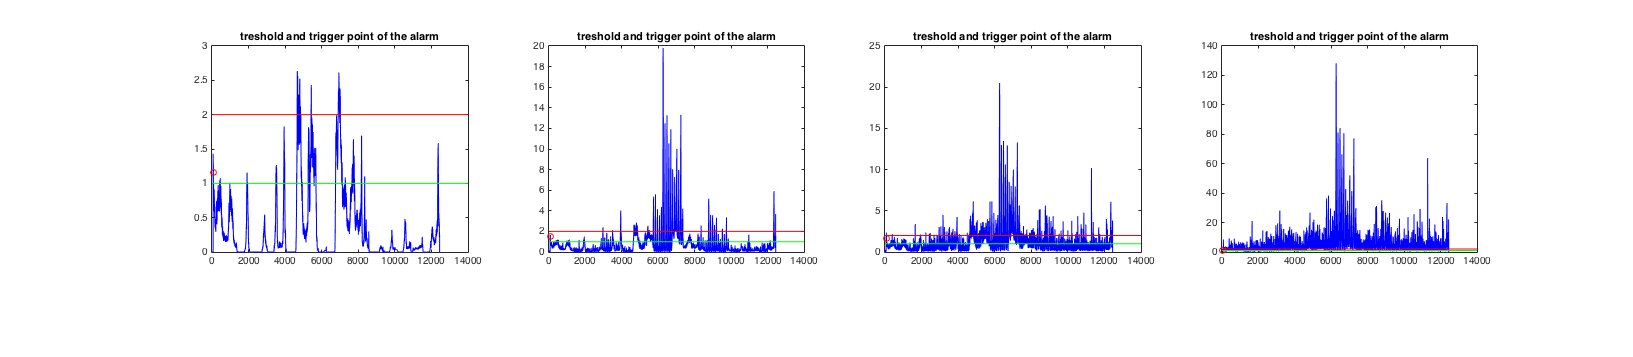
\includegraphics[width=1.5\textwidth]{sections/newFigures/bc1_unfilt_crop.png}}
  \caption{Baby crying.wav, simple algorithm}
  \label{fig:bc1_simp_crop}
\end{figure}

The test results from the \emph{Baby crying.wav} set, Figure
\ref{fig:bc1_simp}, show that the alarm was set off in approximate same time in
every configuration and the reason for this could be that there is a high
energy baby sound in the beginning of all of the files. The \emph{clean} and
the \emph{bird and ventilation} configurations can be considered as plausibly
successful results since the noise levels are not interfering as much as the
two, to the right, configurations.

\begin{figure}[H]
  \centering
  %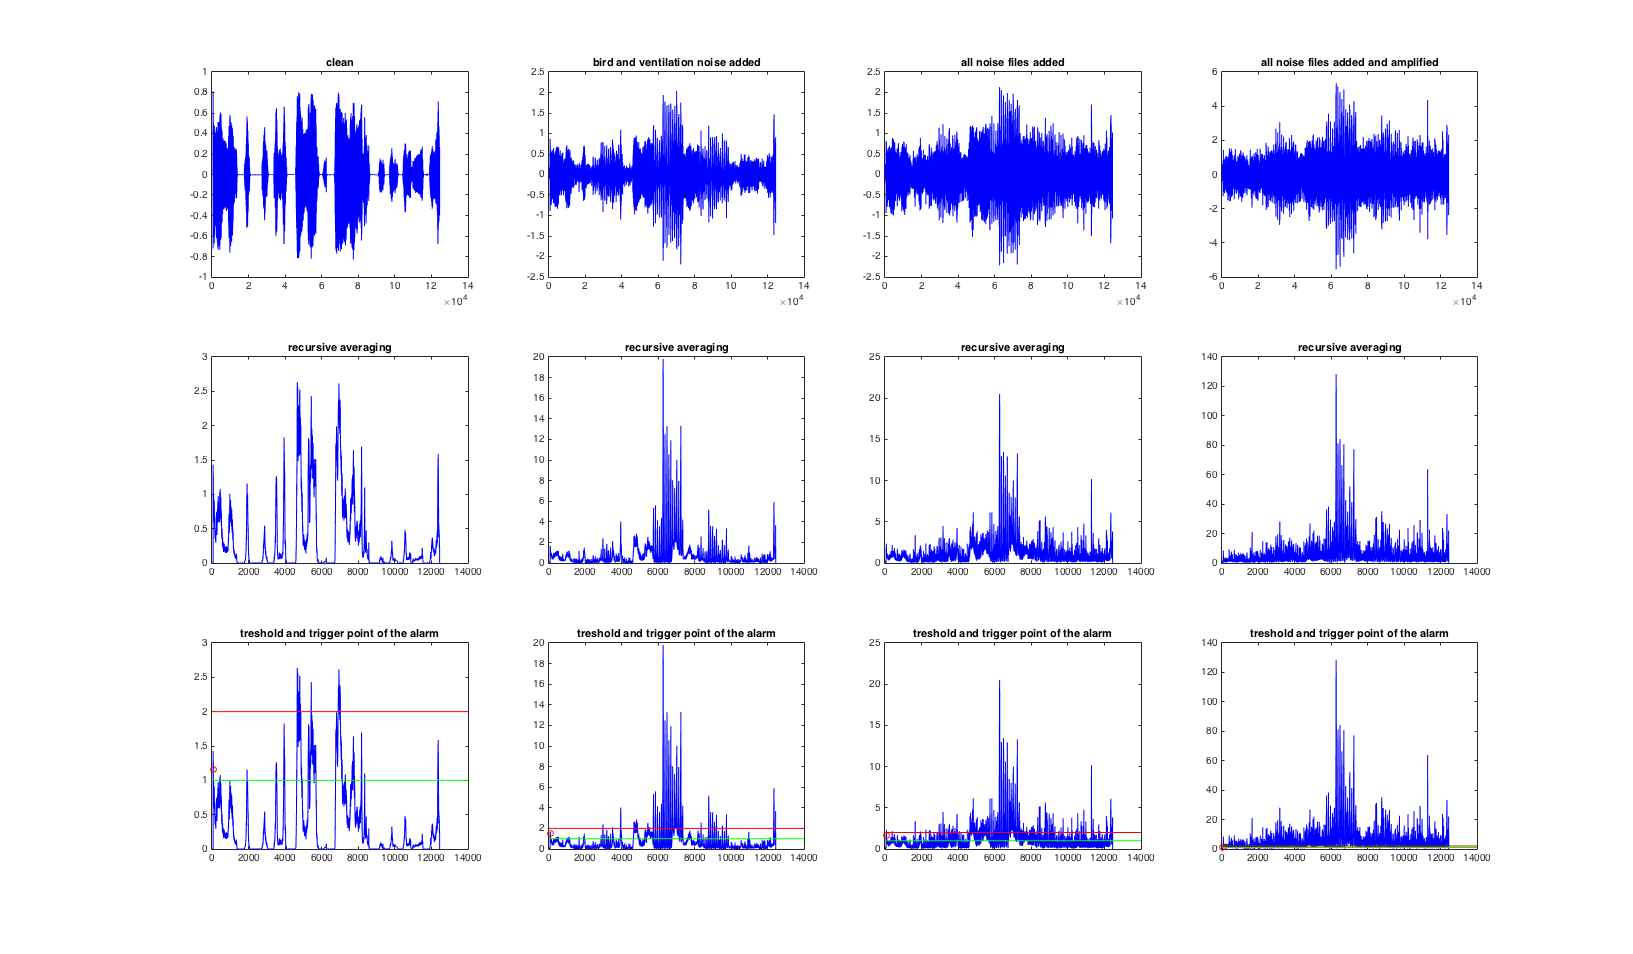
\includegraphics[width=1\textwidth]{sections/newFigures/bc1_unfilt.png}
  \makebox[\textwidth][c]{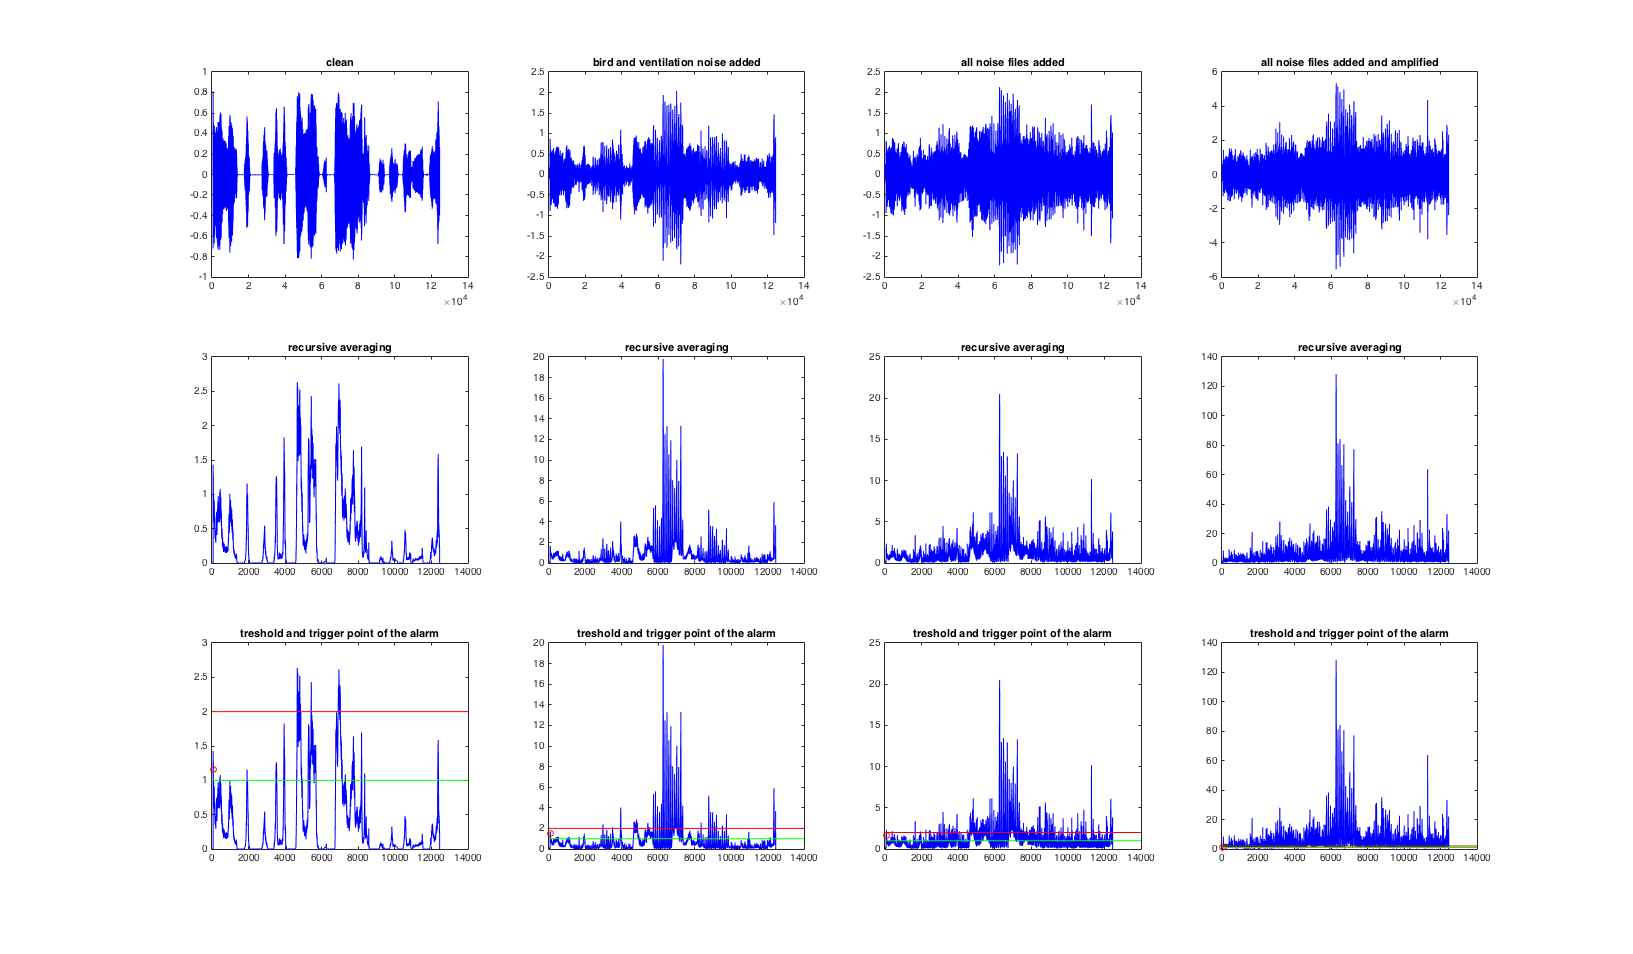
\includegraphics[width=1.5\textwidth]{sections/newFigures/bc1_unfilt.png}}
  \caption{Baby crying.wav, simple algorithm}
  \label{fig:bc1_simp}
\end{figure}

Both \emph{Baby crying1.wav} and \emph{Baby talking.wav} gave unsatisfactory
results without any amplification, as can be seen in Figure \ref{fig:bc2_simp}
and Figure \ref{fig:bt_simp}. The success of setting of the alarm in the other
configurations were due to the noise.. Not remotely close to trigger the alarm
in clean configuration, illustrated be the left most plots, the test were
performed a second time with amplified baby sound.

\begin{figure}[H]
  \centering
  %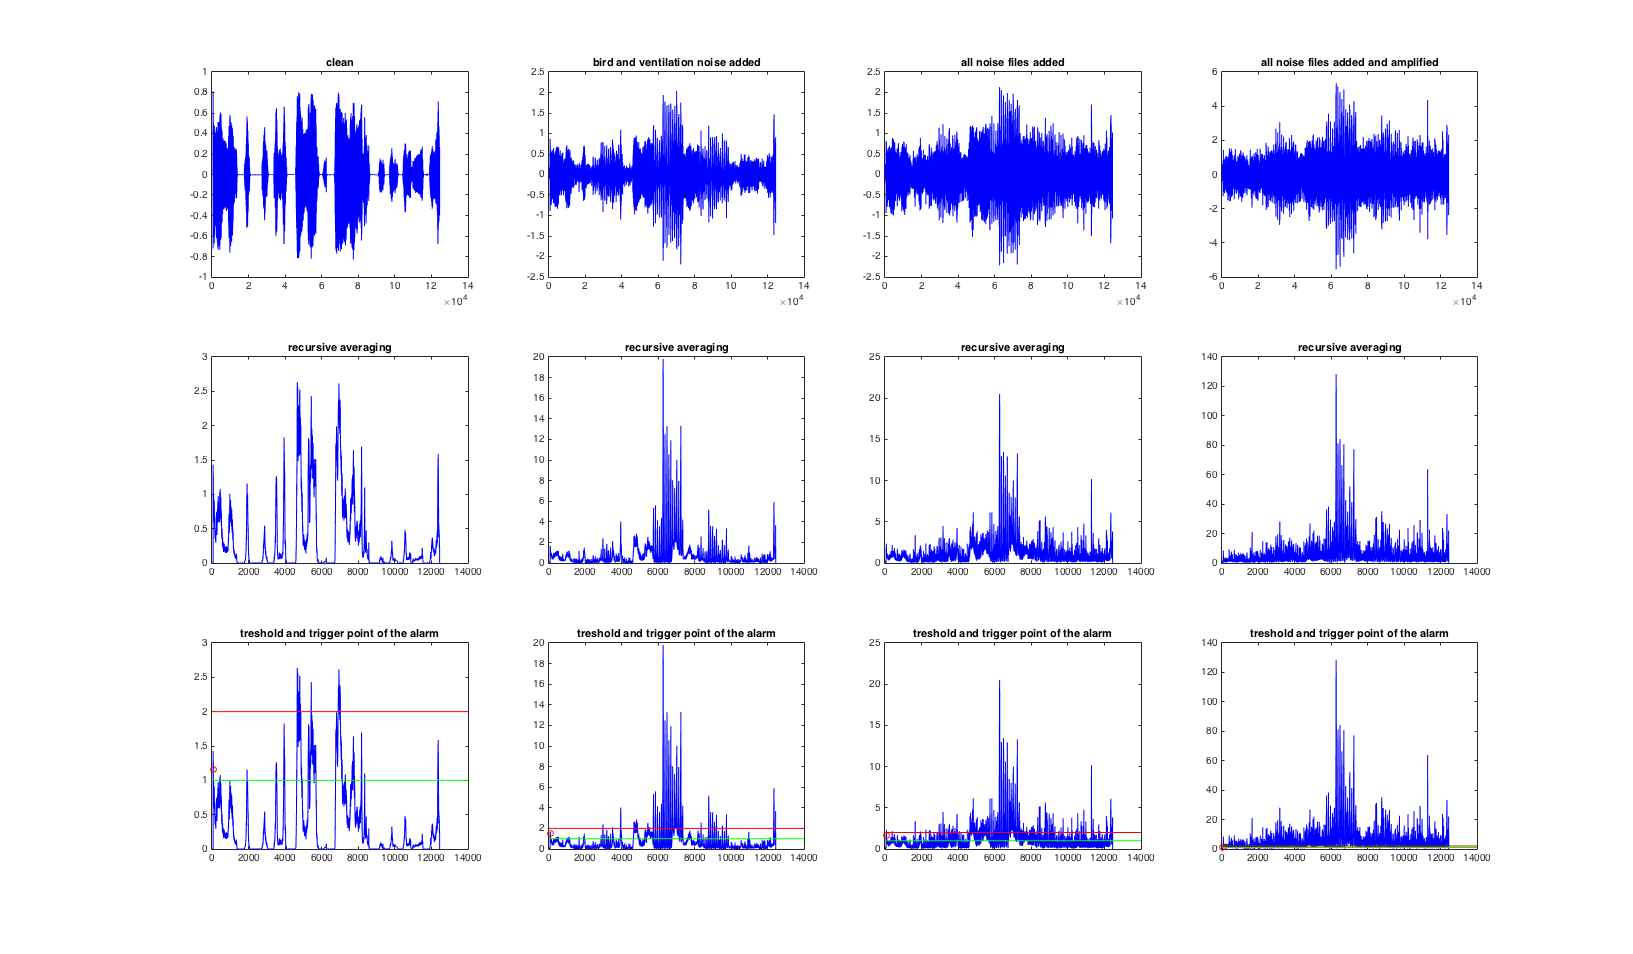
\includegraphics[width=1\textwidth]{sections/newFigures/bc1_unfilt.png}
  \makebox[\textwidth][c]{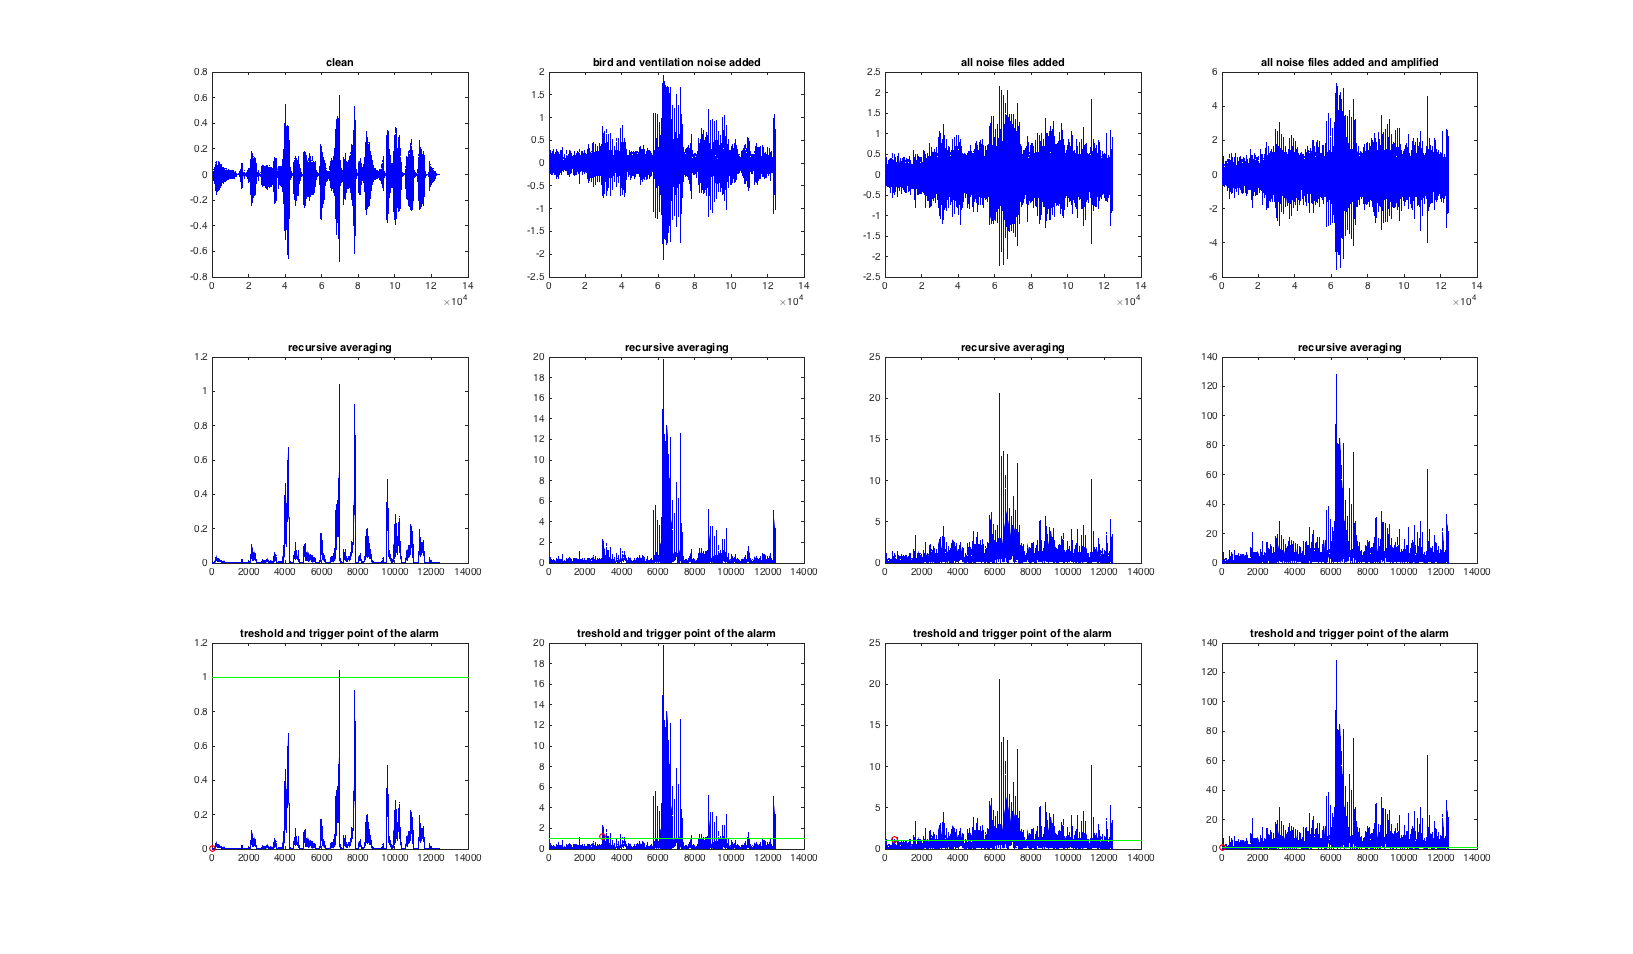
\includegraphics[width=1.5\textwidth]{sections/newFigures/bc2_unfilt.png}}
  \caption{Baby crying1.wav, simple algorithm}
  \label{fig:bc2_simp}
\end{figure}
\begin{figure}[H]
  \centering
  %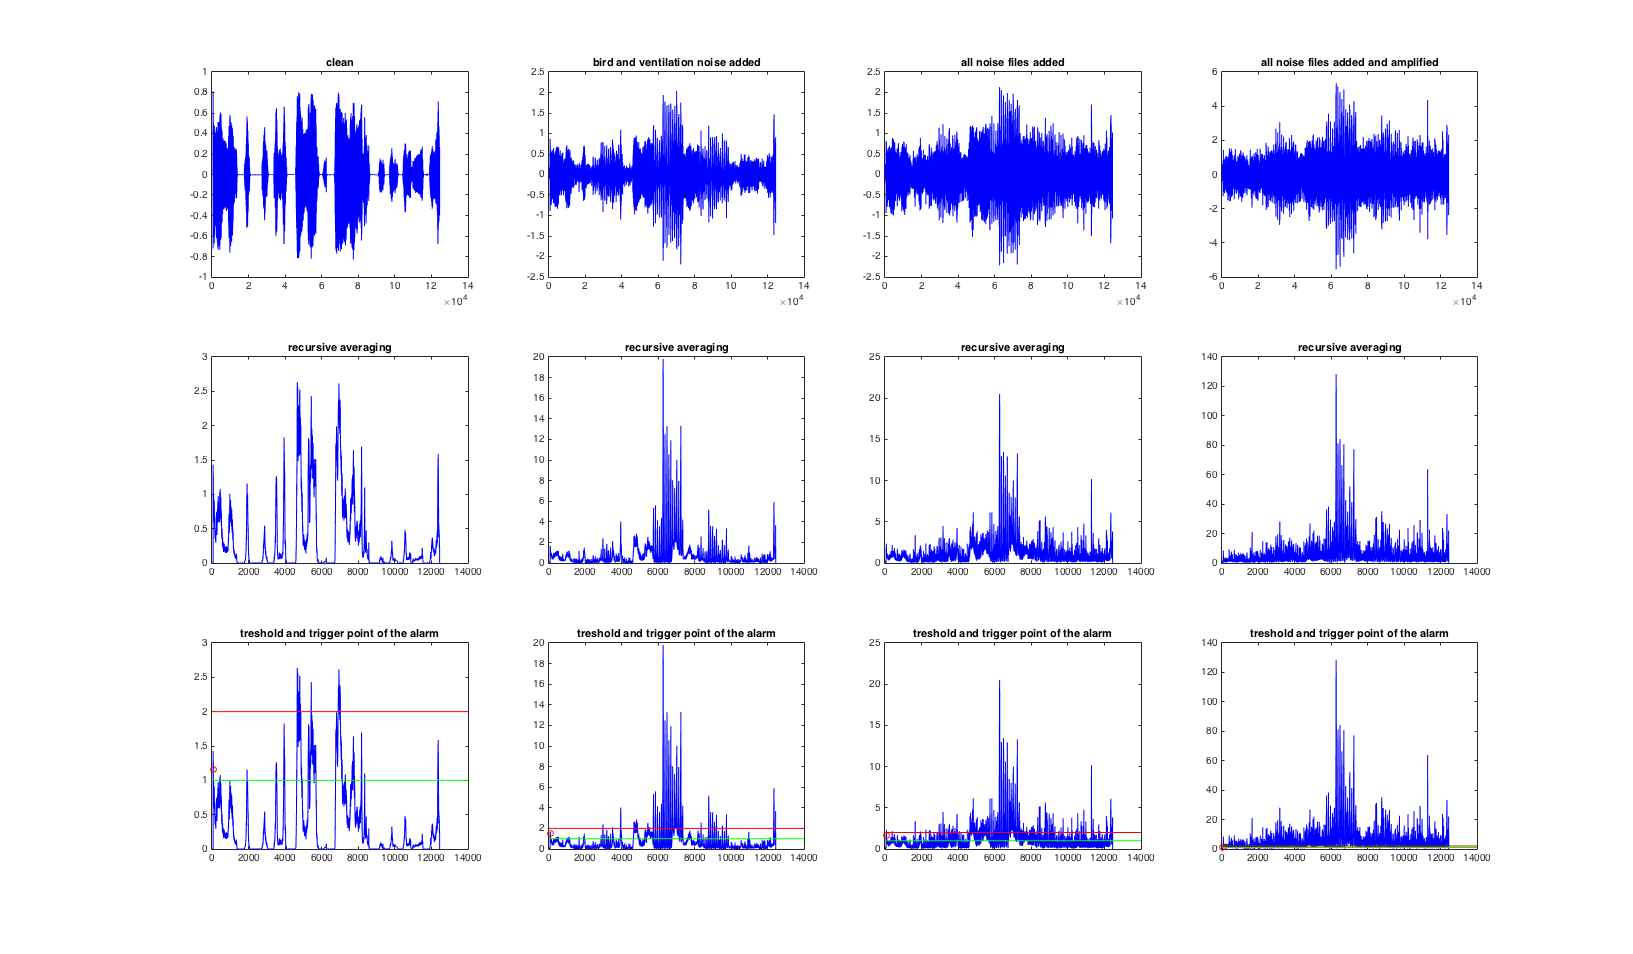
\includegraphics[width=1\textwidth]{sections/newFigures/bc1_unfilt.png}
  \makebox[\textwidth][c]{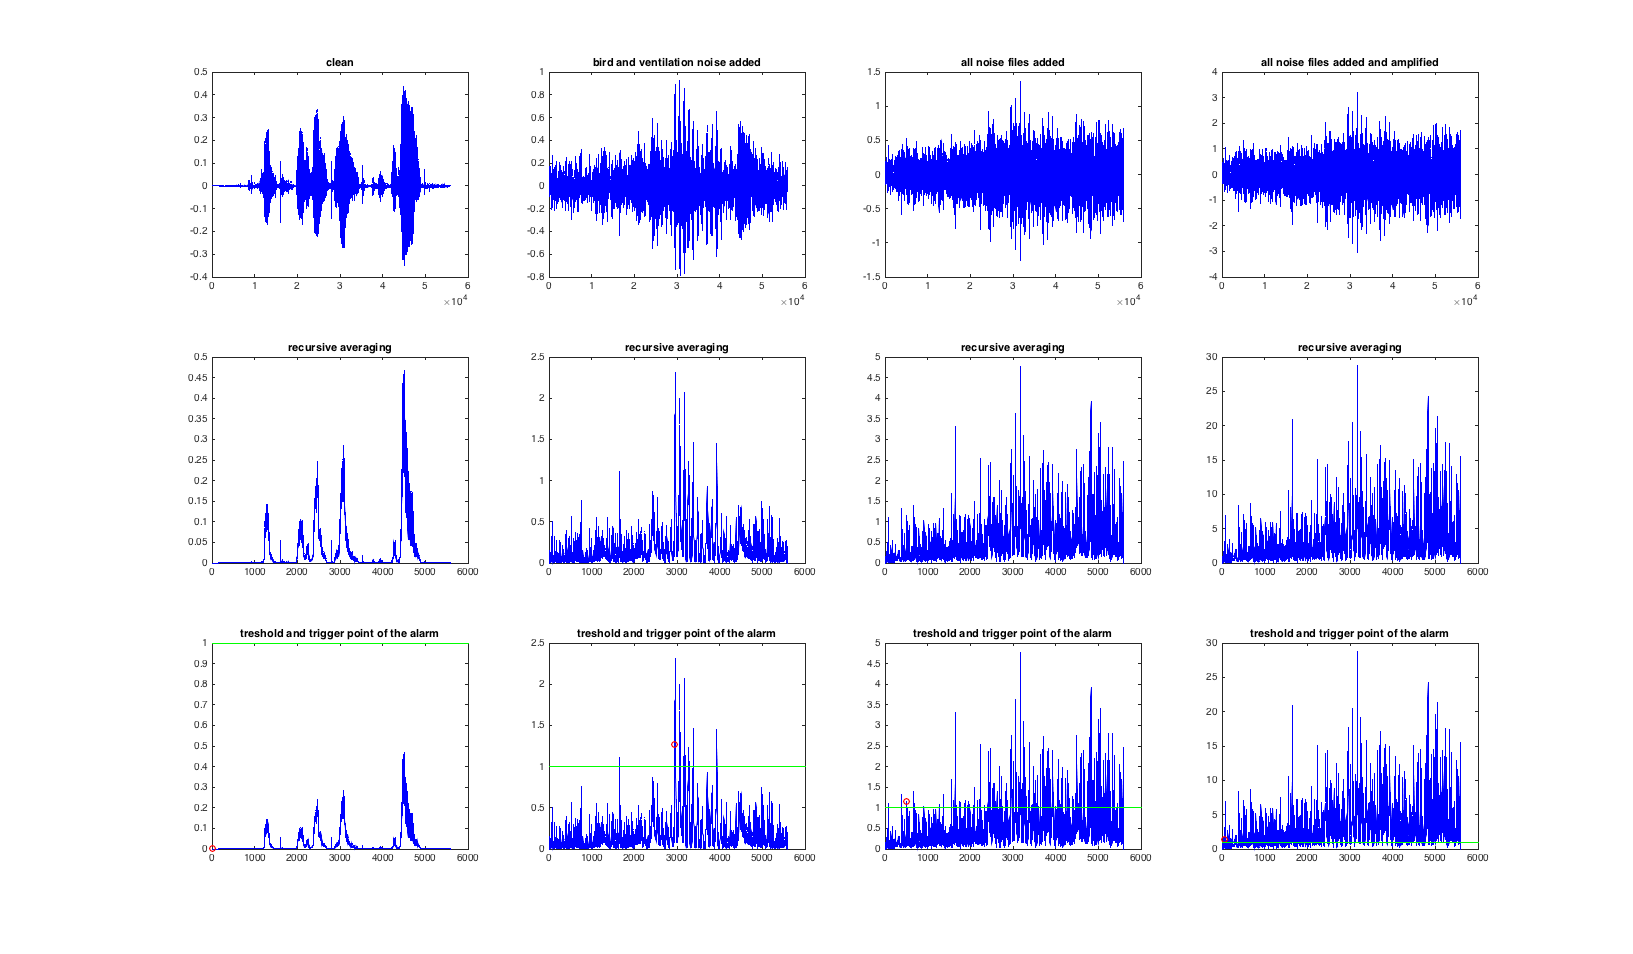
\includegraphics[width=1.5\textwidth]{sections/newFigures/bt_unfilt.png}}
  \caption{Baby talking.wav, simple algorithm}
  \label{fig:bt_simp}
\end{figure}

By having the baby sounds amplified before the noise is added, making sure that
the alarm sets off in clean configuration, gives a possibility for the baby
sounds to trigger the alarm in other configurations as well, see Figure
\ref{fig:bc2_simp_amped} and Figure \ref{fig:bt_simp_amped}.  Unfortunately,
the simple algorithm performed poorly for the \emph{Baby crying1.wav}
set, Figure \ref{fig:bc2_simp_amped}, but in the \emph{Baby
talking.wav} set, Figure \ref{fig:bt_simp_amped}, the first two
configurations, \emph{clean} and \emph{bird and ventilation},
performed surprisingly well.

\begin{figure}[H]
  \centering
  %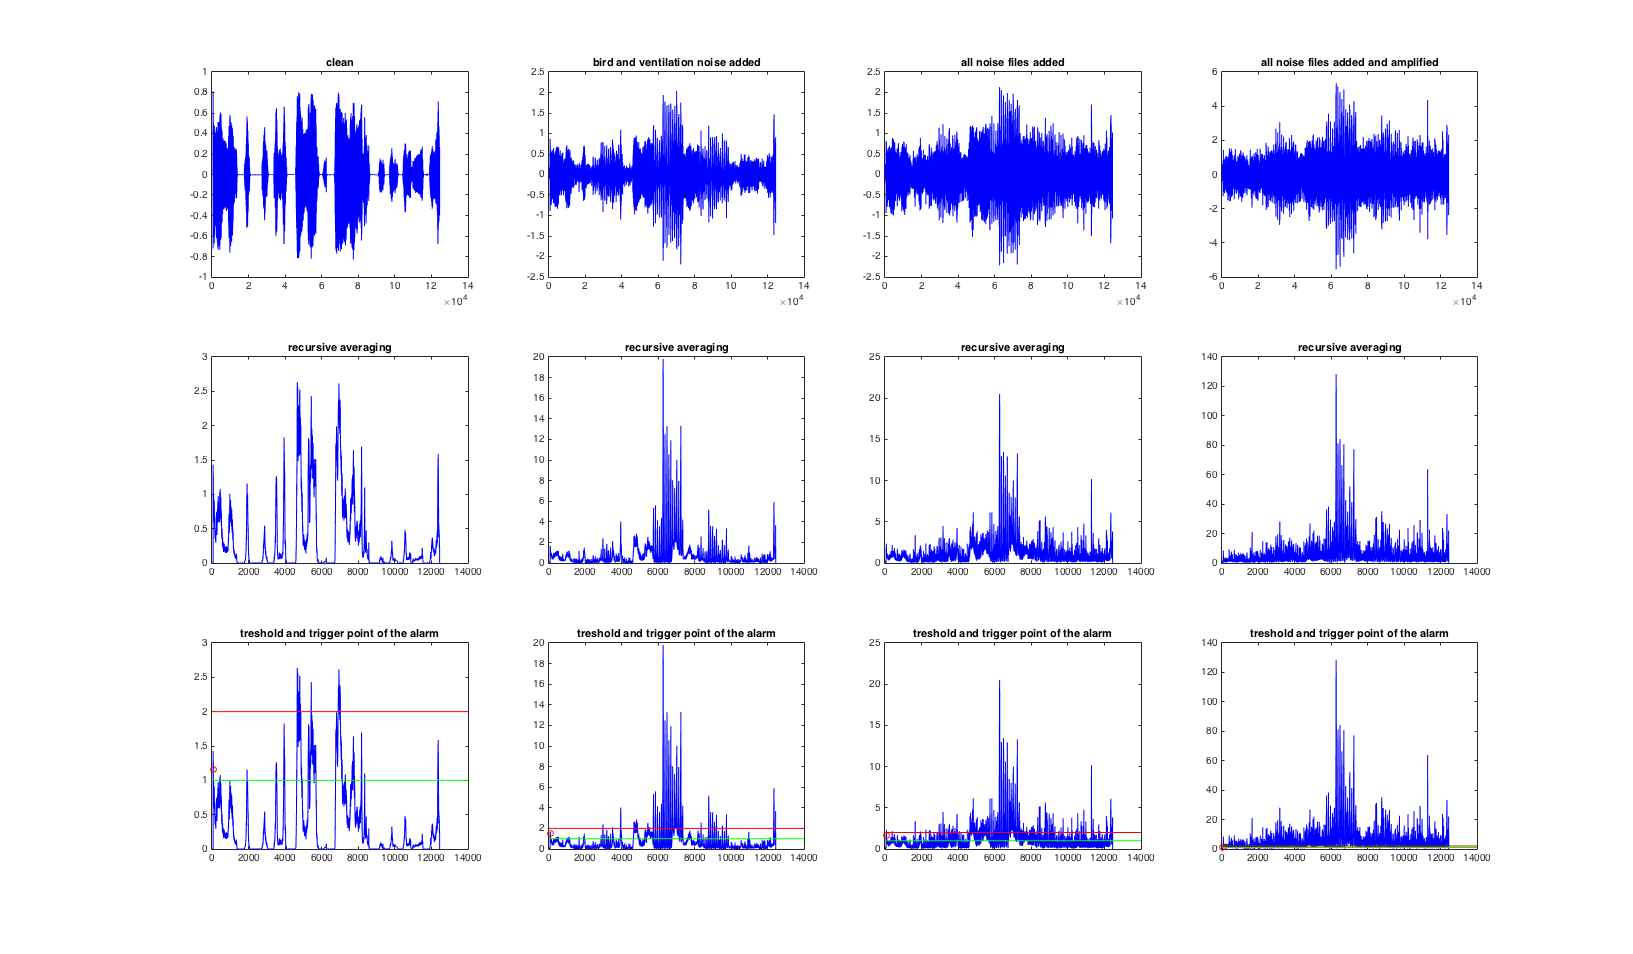
\includegraphics[width=1\textwidth]{sections/newFigures/bc1_unfilt.png}
  \makebox[\textwidth][c]{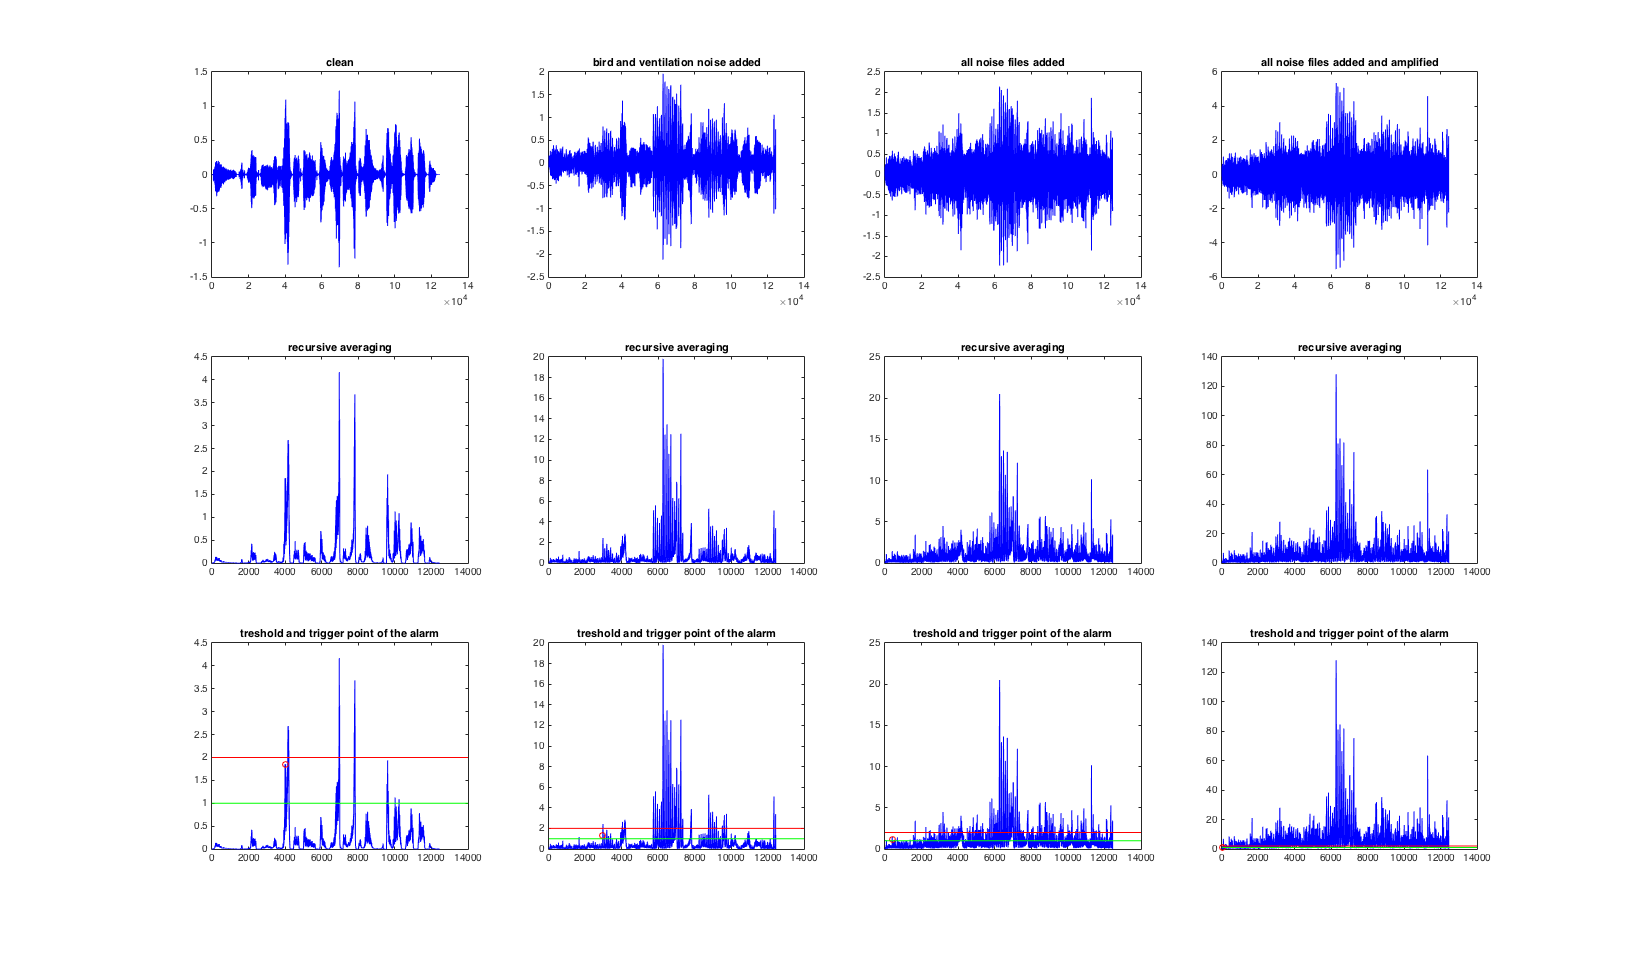
\includegraphics[width=1.5\textwidth]{sections/newFigures/bc2_unfilt_amped.png}}
  \caption{Amplified Baby crying1.wav, simple algorithm}
  \label{fig:bc2_simp_amped}
\end{figure}
\begin{figure}[H]
  \centering
  %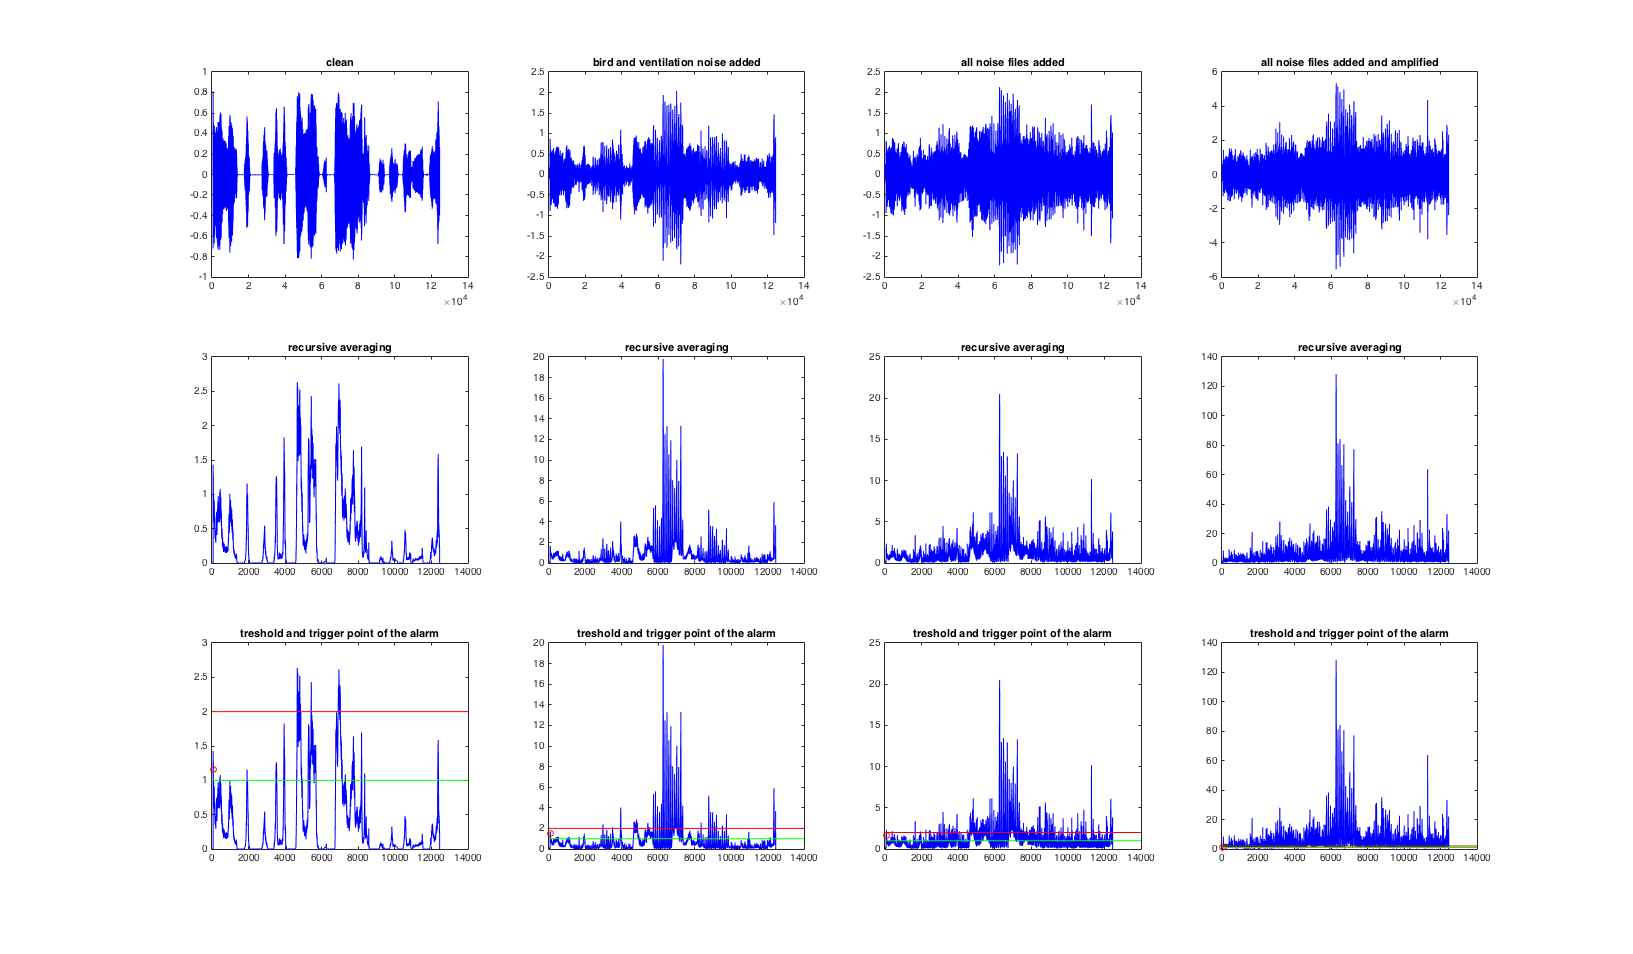
\includegraphics[width=1\textwidth]{sections/newFigures/bc1_unfilt.png}
  \makebox[\textwidth][c]{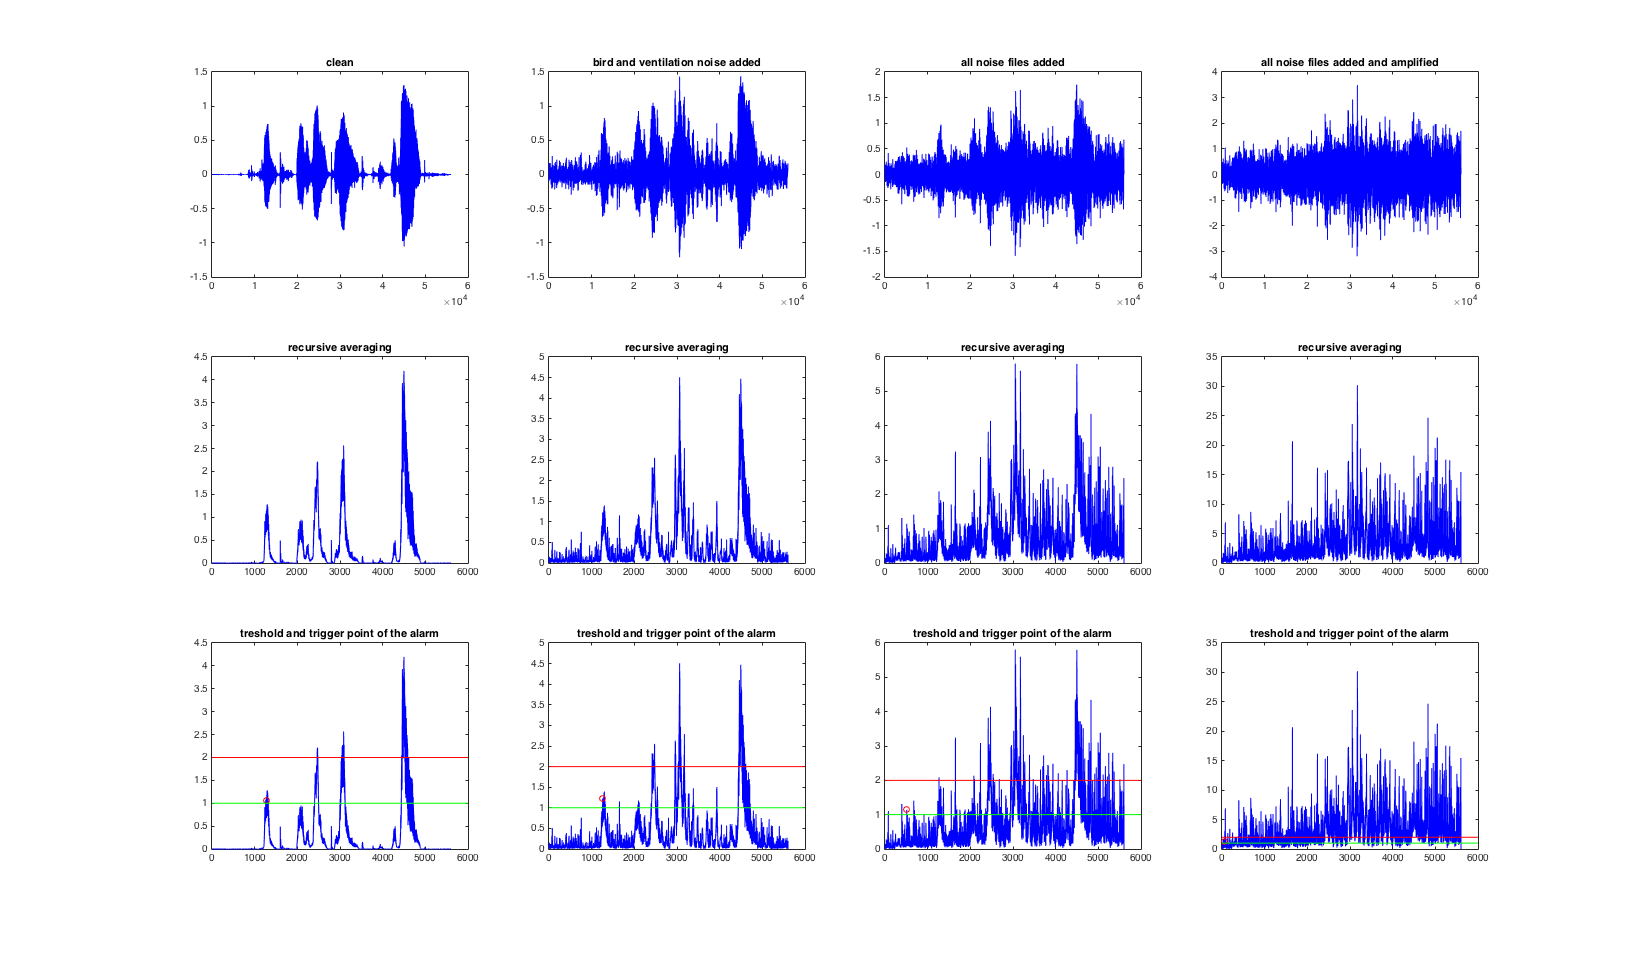
\includegraphics[width=1.5\textwidth]{sections/newFigures/bt_unfilt_amped.png}}
  \caption{Amplified Baby talking.wav, simple algorithm}
  \label{fig:bt_simp_amped}
\end{figure}

The advanced algorithm performed, as expected, exceptionally well due to
unwanted frequencies being suppressed, not interfering with the power
calculations. Figure \ref{fig:bc1_advn}, Figure \ref{fig:bc2_advn_amped} and
Figure \ref{fig:bt_advn_amped} show great results, except for the early trigger 
in the last configuration of the \emph{Baby talking.wav} set. The alarm was set
off earlier because the signal was infected with noise. Despite the early
trigger of the alarm, it was executed during baby activity and not by the added
noise. The alarm could have been triggered during the same time in other
configurations of that set as well.

\begin{figure}[H]
  \centering
  %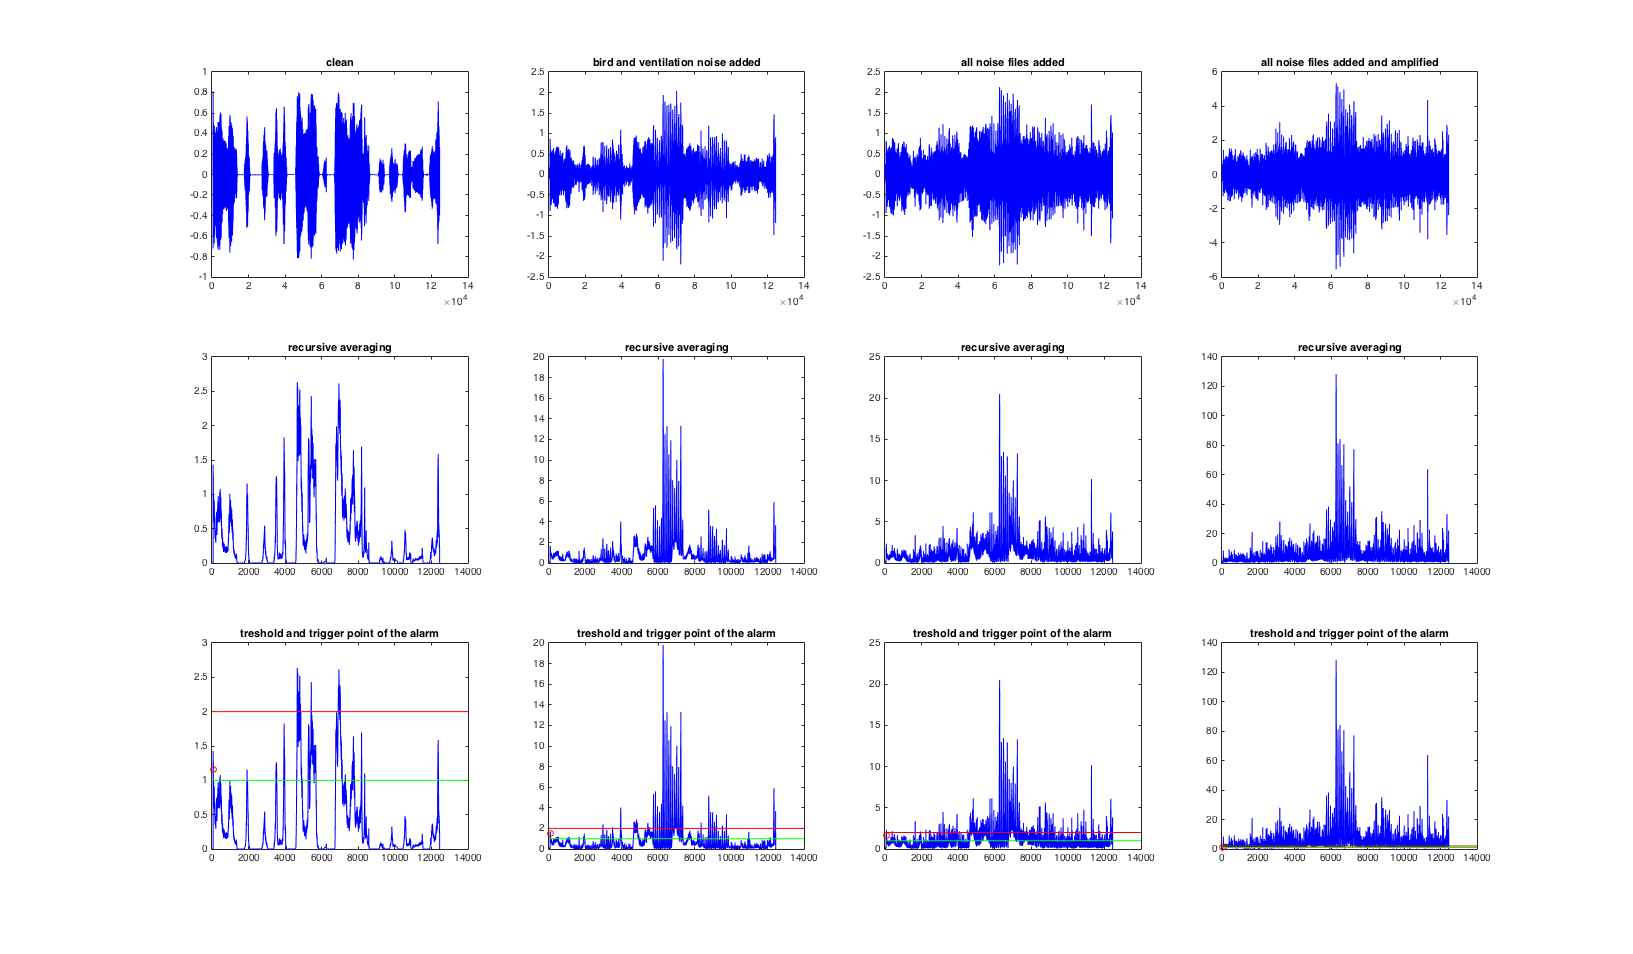
\includegraphics[width=1\textwidth]{sections/newFigures/bc1_unfilt.png}
  \makebox[\textwidth][c]{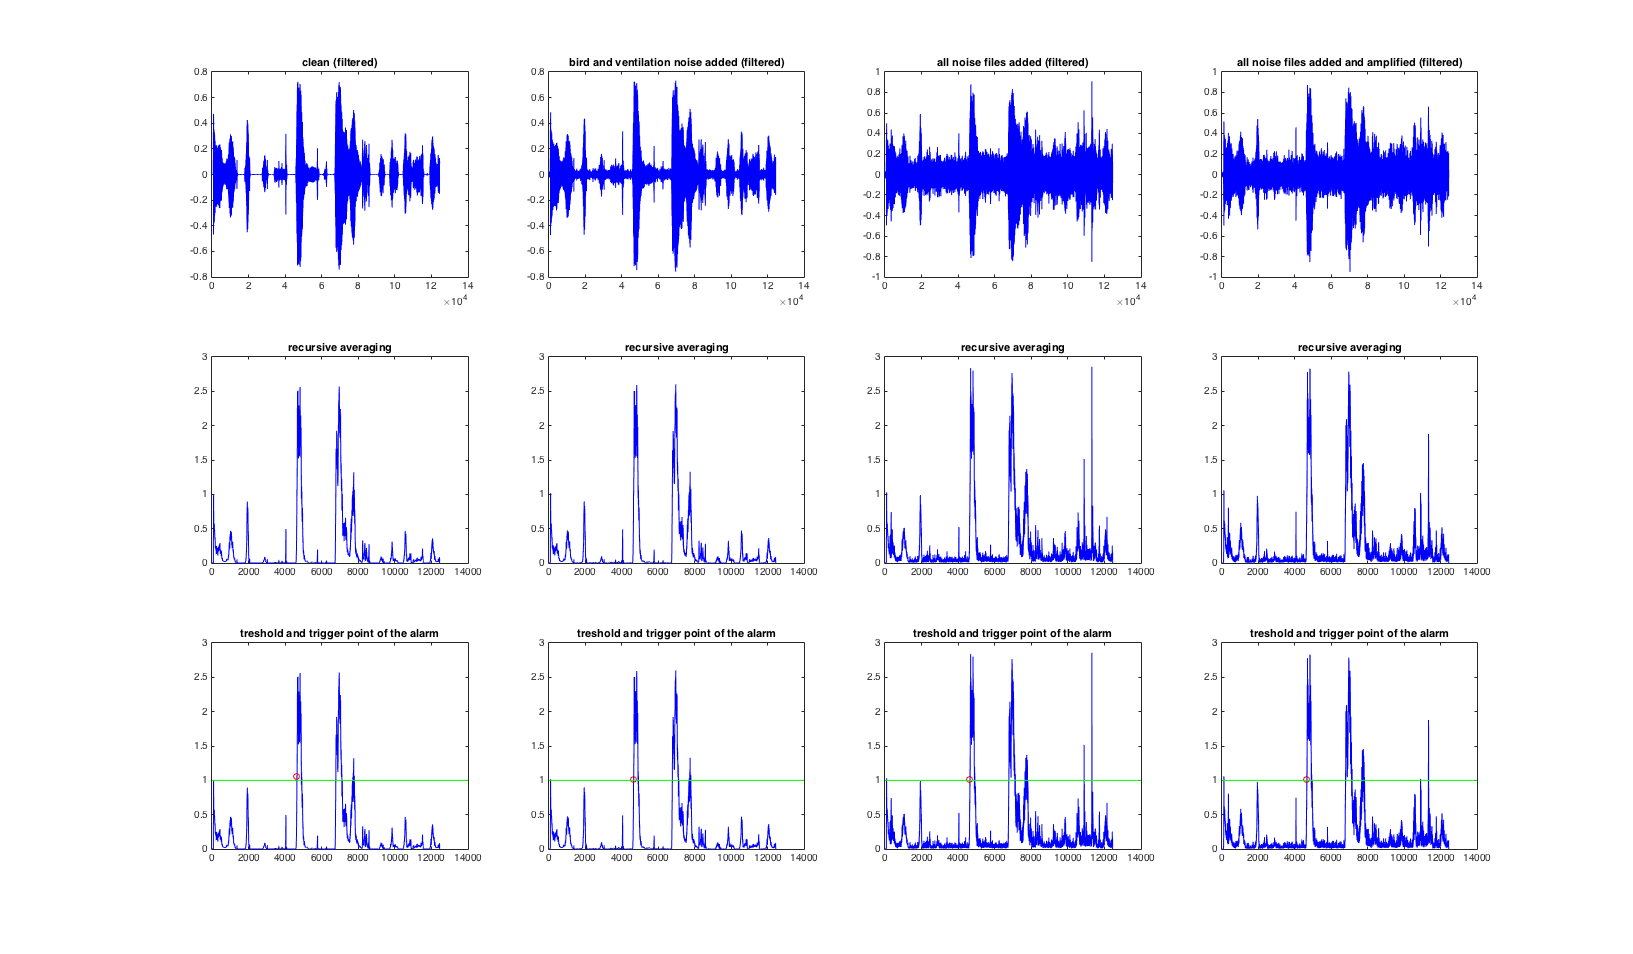
\includegraphics[width=1\textwidth]{sections/newFigures/bc1_filt.png}}
  \caption{Baby crying.wav, advanced algorithm}
  \label{fig:bc1_advn}
\end{figure}
\begin{figure}[H]
  \centering
  %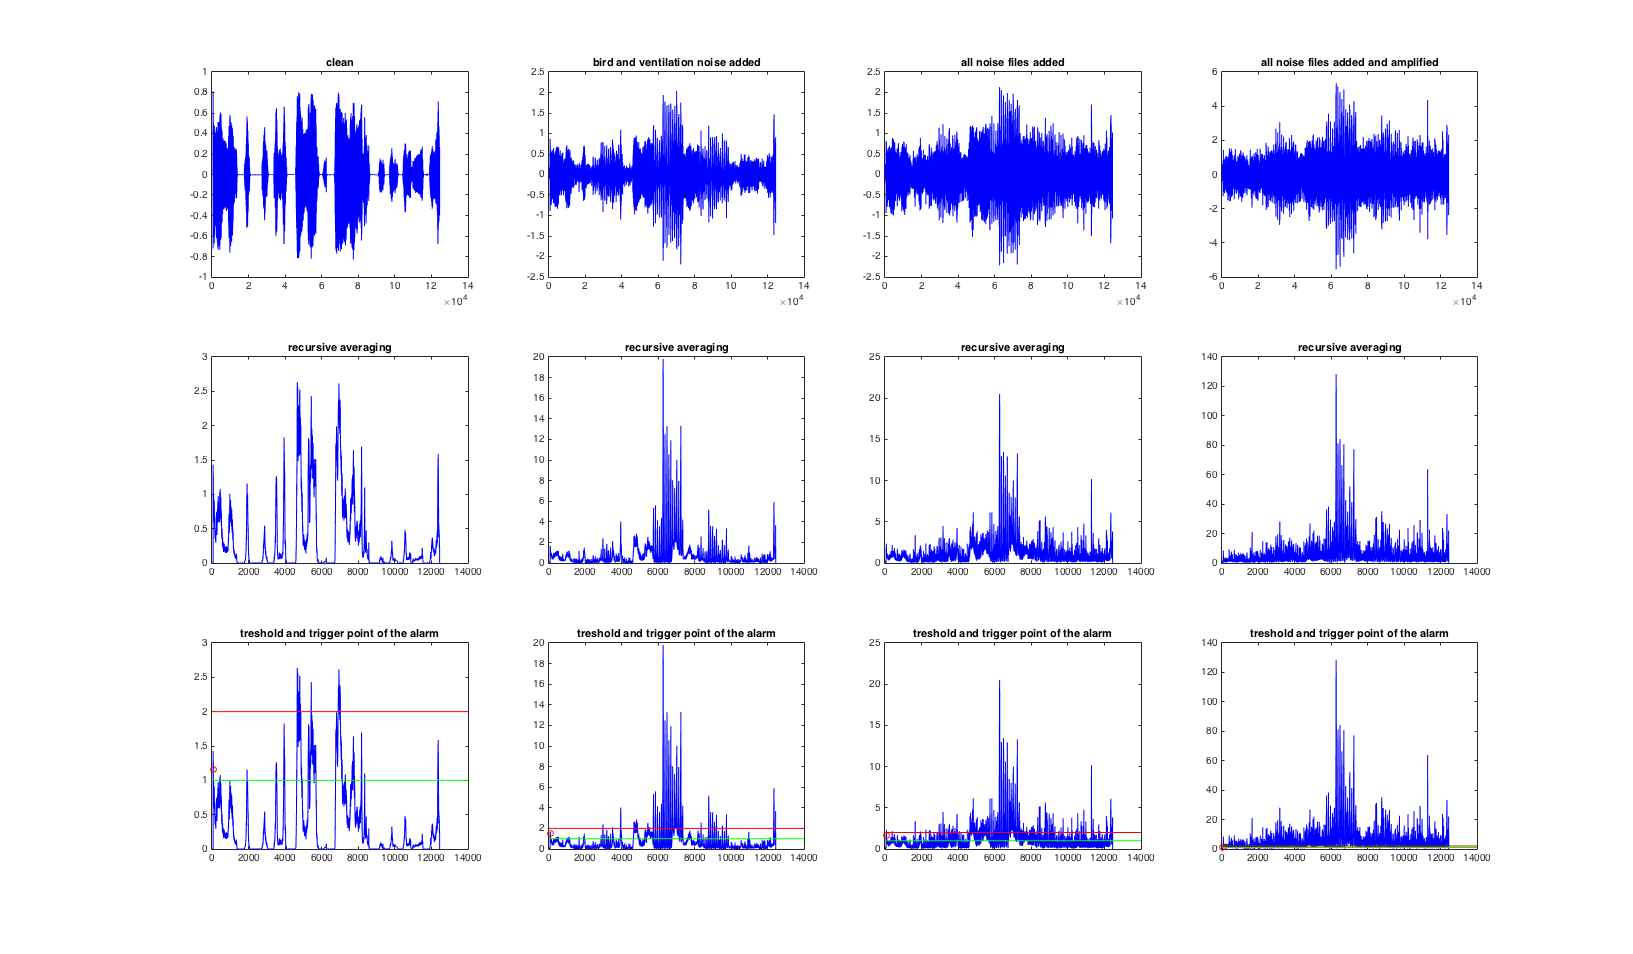
\includegraphics[width=1\textwidth]{sections/newFigures/bc1_unfilt.png}
  \makebox[\textwidth][c]{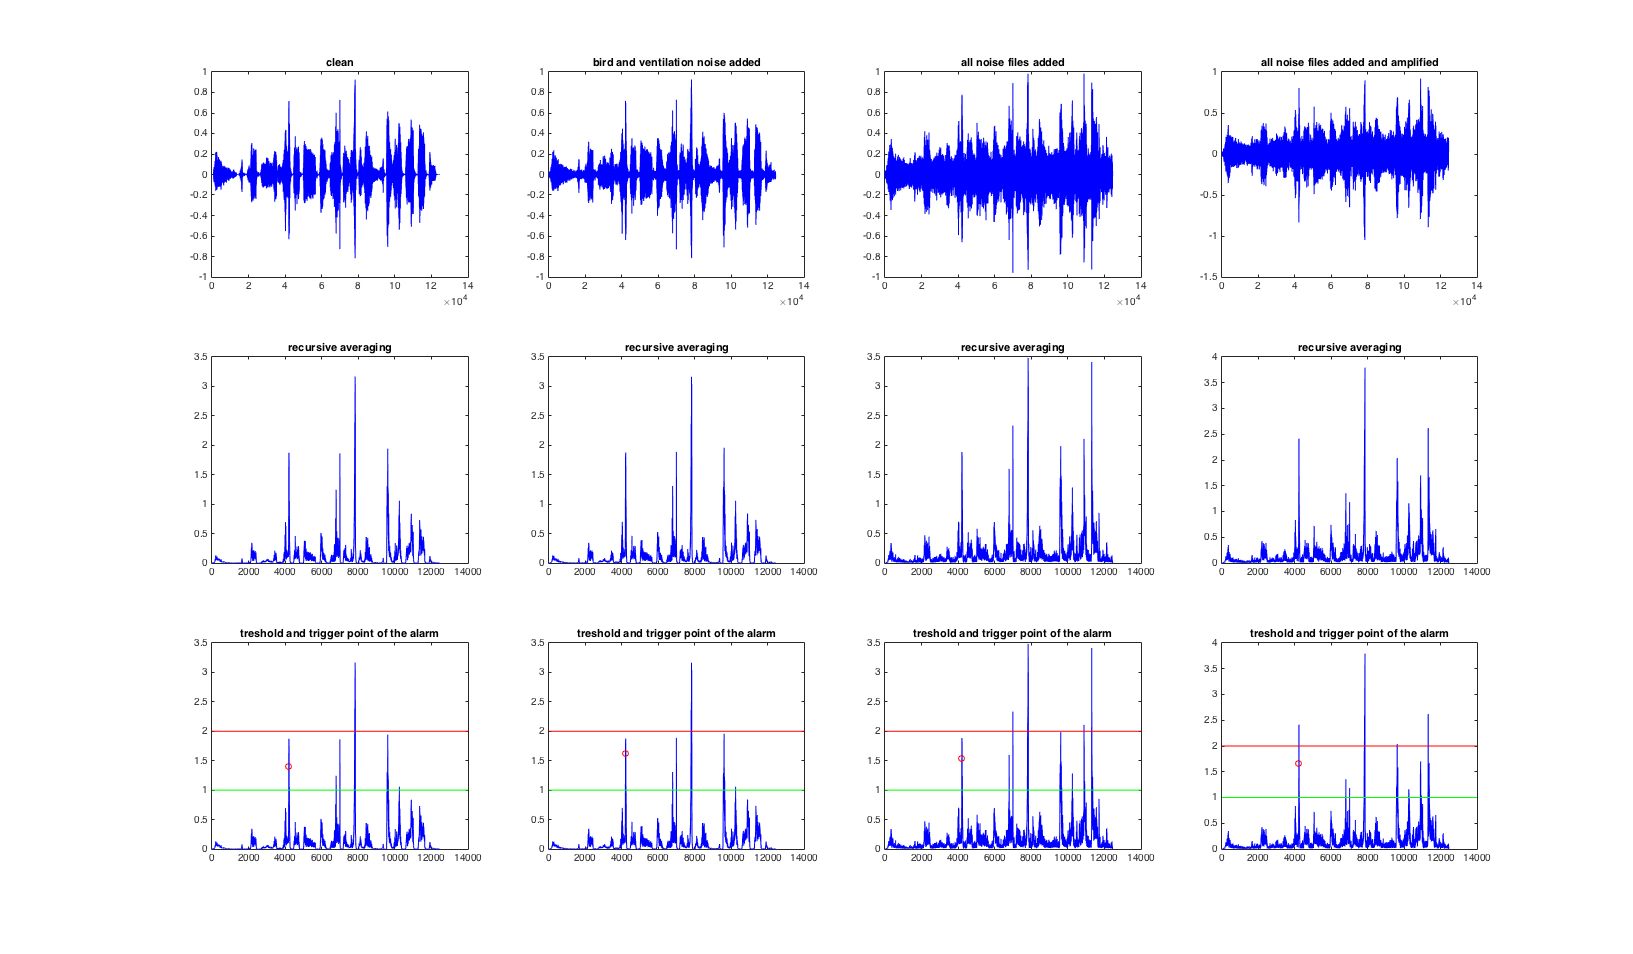
\includegraphics[width=1\textwidth]{sections/newFigures/bc2_filt_amped.png}}
  \caption{Amplified Baby crying1.wav, advanced algorithm}
  \label{fig:bc2_advn_amped}
\end{figure}
\begin{figure}[H]
  \centering
  %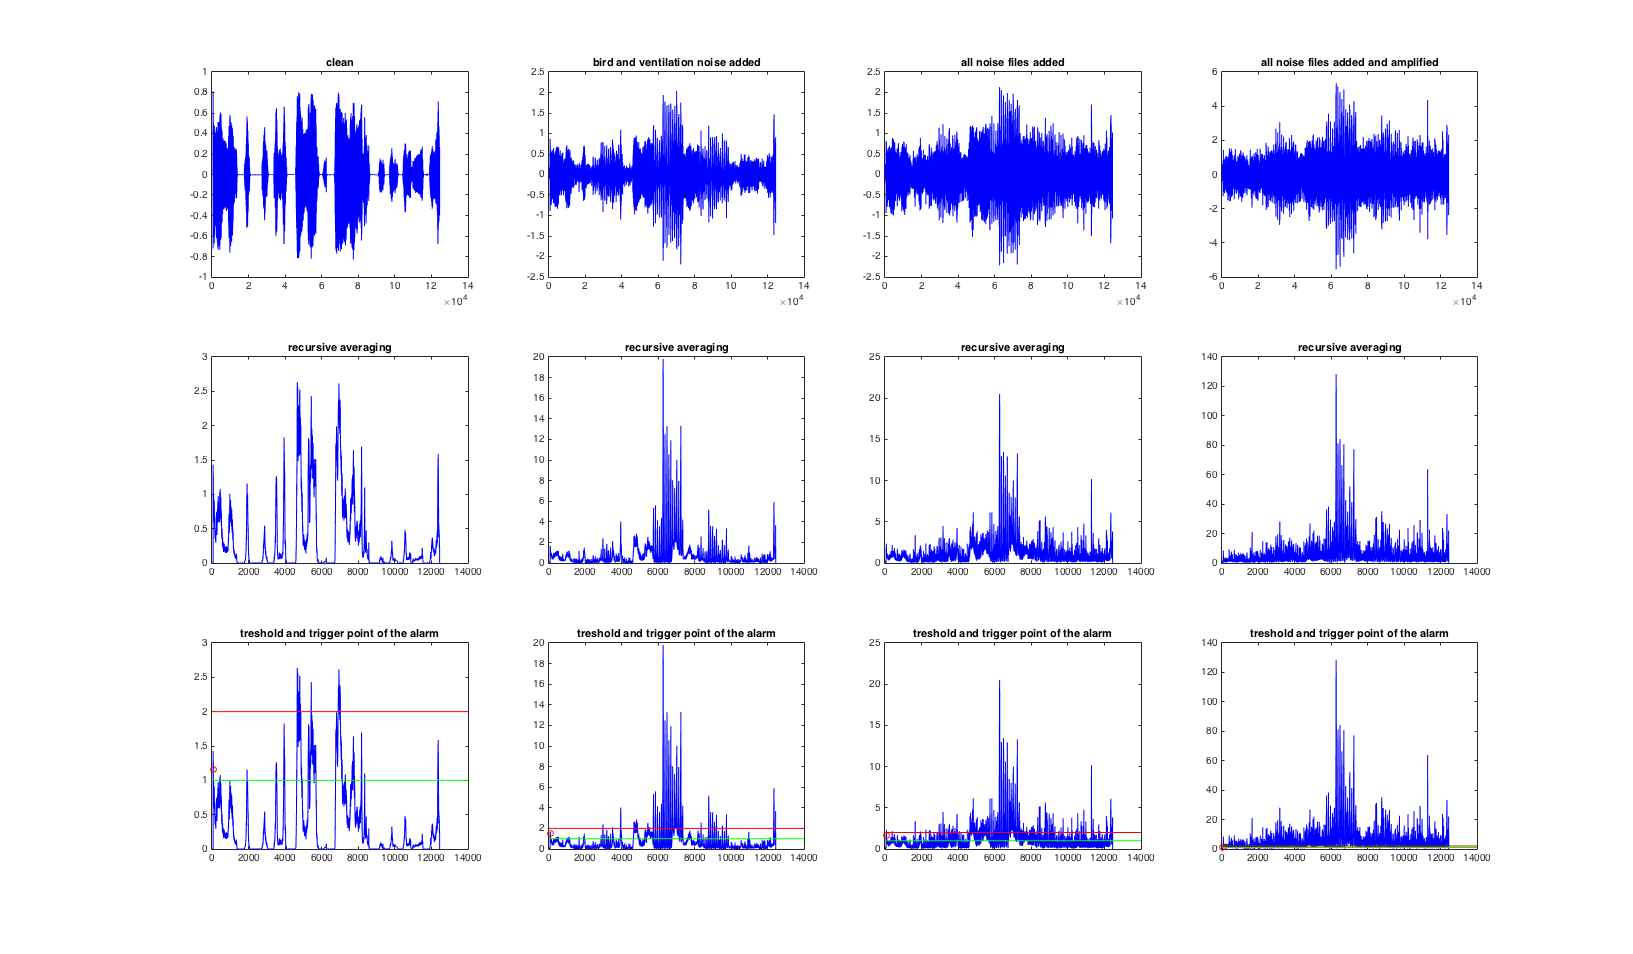
\includegraphics[width=1\textwidth]{sections/newFigures/bc1_unfilt.png}
  \makebox[\textwidth][c]{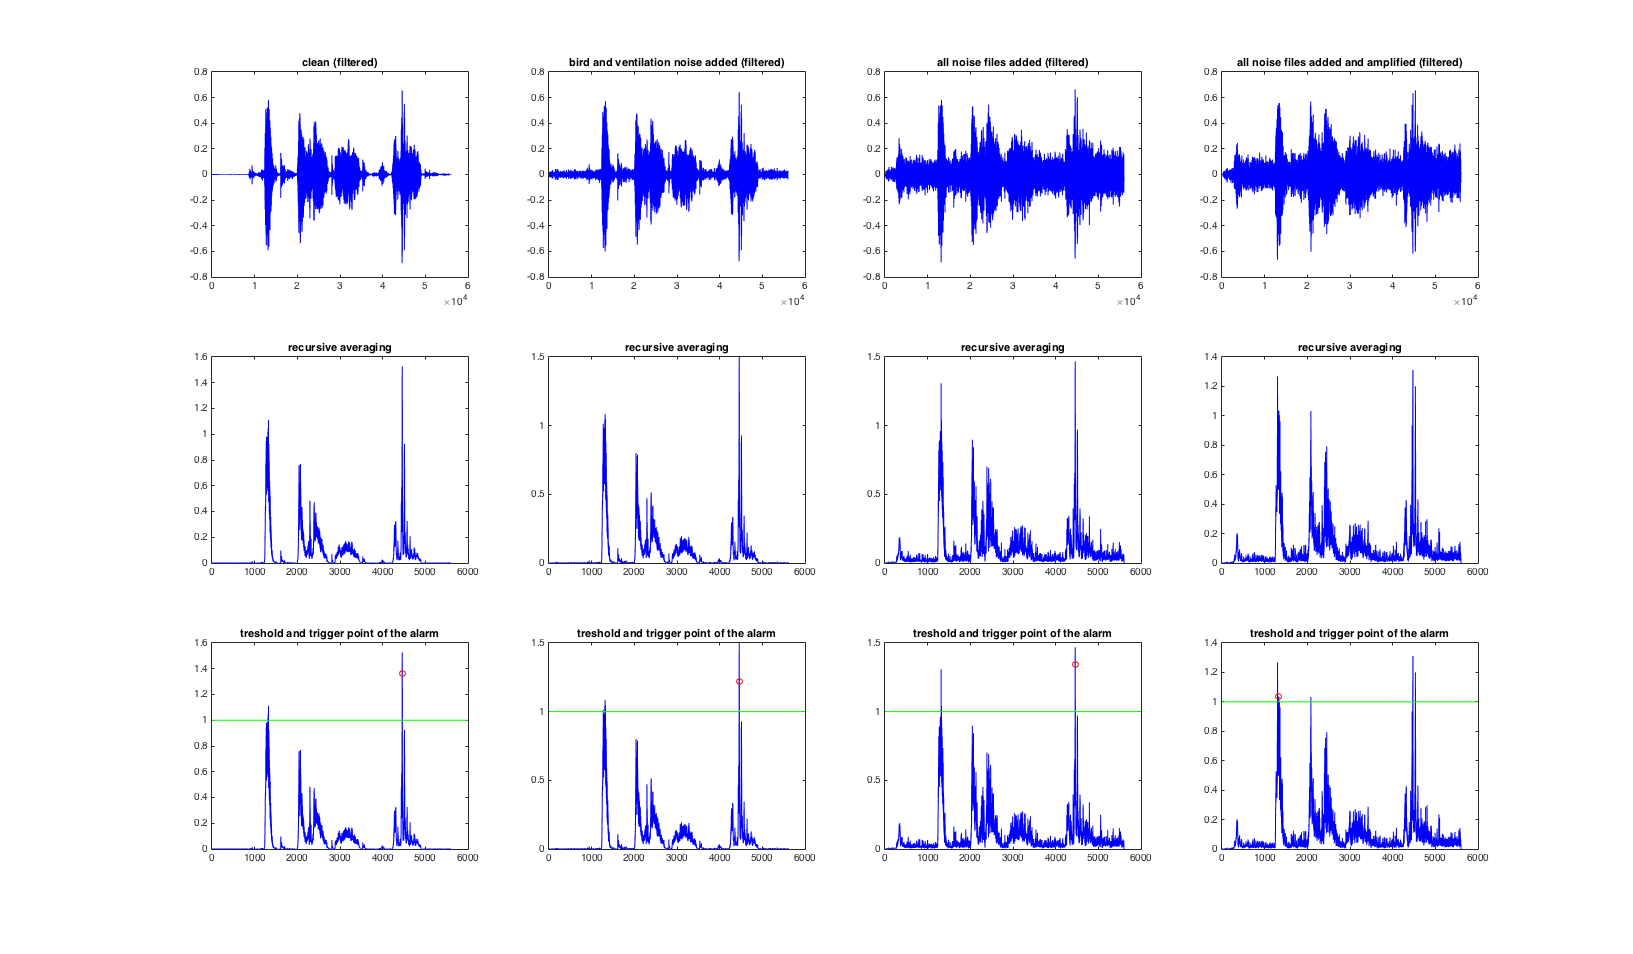
\includegraphics[width=1\textwidth]{sections/newFigures/bt_filt_amped.png}}
  \caption{Amplified Baby talking.wav, advanced algorithm}
  \label{fig:bt_advn_amped}
\end{figure}

\subsection{Conclusion}
Giving the results from the two different algorithms, it is fair to state the
simple algorithm was unreliable since the noise levels could trigger the alarm.
If the design goal is accuracy, reliability and good performance for the BAD
application then implementing the advanced algorithm would be the best option.
However, both algorithms rely on the \emph{recursive averaging} algorithm.
Implementing it must be done either way and should this be done within short
amount of time, an attempt should be preformed to implement the Butterworth
bandpass filter. If the filter issue can not be overcome with built-in Java
classes, third-party libraries, or guidelines from the institute then the
advanced algorithm will not be implemented. This should be considered as bonus
task for Part 3 of the course.
